\section{How to Use}
This programm allows you to open a json of toml file containing an elk graph and shows an animation of the selected cycle breaking process used on the graph.
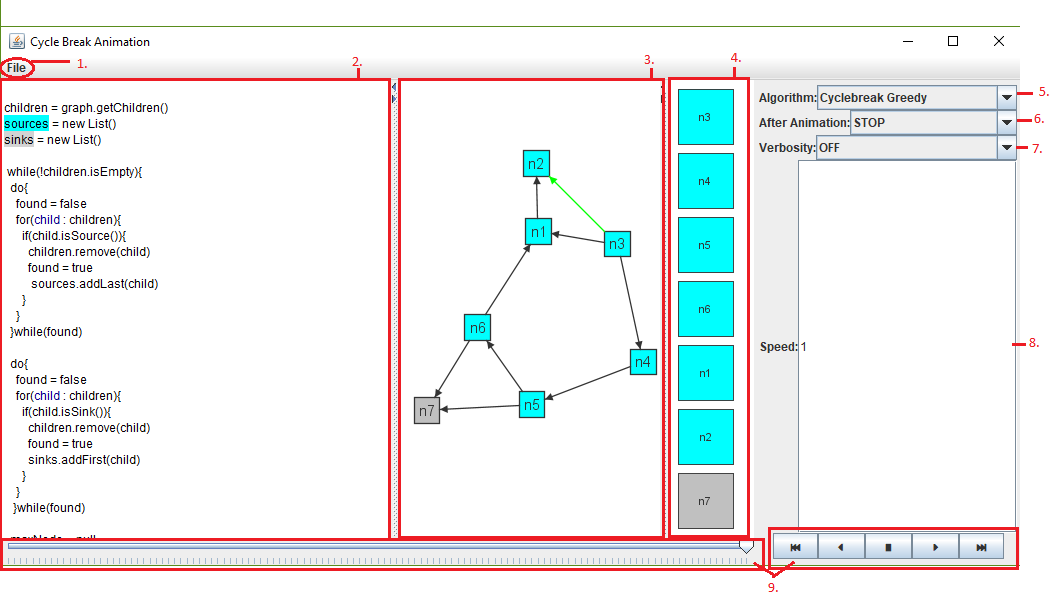
\includegraphics[width=\textwidth]{parts/InterfaceV2_1}

\begin{list}{-}{}
\item[1.] You can choos a file from the filesystem to be diplayed and you can save an animation for a loaded graph as a gif here
\item[2.] The current choosen algorithm is displayed here in pseudocode
\item[3.] A visual representation of the loaded full graph
\item[4.] A topological representation representation of the loaded graph
\item[5.] A list to choose a cycle break algorithm
\item[6.] Choose what should be done when autoplay reaches an end
\begin{list}{-}{}
\item[STOP] End the animation
\item[LOOP] Start the animation from the beginning
\item[REVERSE] Play the animation reversed
\end{list}
\item[7.] Choose verbosity of the steps of the animation
\begin{list}{-}{}
\item[OFF] Step funktion is disabled
\item[DEPTH 0-6] Steps stop when they reach the indent of the pseudocode with a number lesser or equal than the number of DEPTH
\end{list}
\item[8.] Set the speed the animation is displayed with
\item[9.] Slider and controls for the animation
\begin{list}{-}{}
\item[SLIDER] Displayes the current progress of the animation can be moved to display specific times in the animation
%\item[ \stepbackwards ]  TODO Unicode
%\item[⏮]
\item[ $| \! \! \! \blacktriangleleft \! \blacktriangleleft$ ] Plays the animation backwards till the Pseudocode reaches an indent set by verbosity
\item[ $\blacktriangleleft$ ] Plays the animation backwards till the end
\item[$ \blacksquare $] Stops the animation
\item[$ \blacktriangleright $] Plays the animation forwards
\item[$ \blacktriangleright \! \blacktriangleright \! \! \!|$]  Plays the animation forwards till the Pseudocode reaches an indent set by verbosity
\end{list}
\end{list}